\section{综述}
JPEG 2000是基于小波变换的图像压缩标准,由Joint Photographic Experts Group组织创建和维护。本次project的目的是复现JPEG 2000的压缩流程,完成一个“自定义”的JPEG 2000压缩程序。其核心编解码模块与过程如下图所示:\par

\begin{figure}[H]
	\centering
	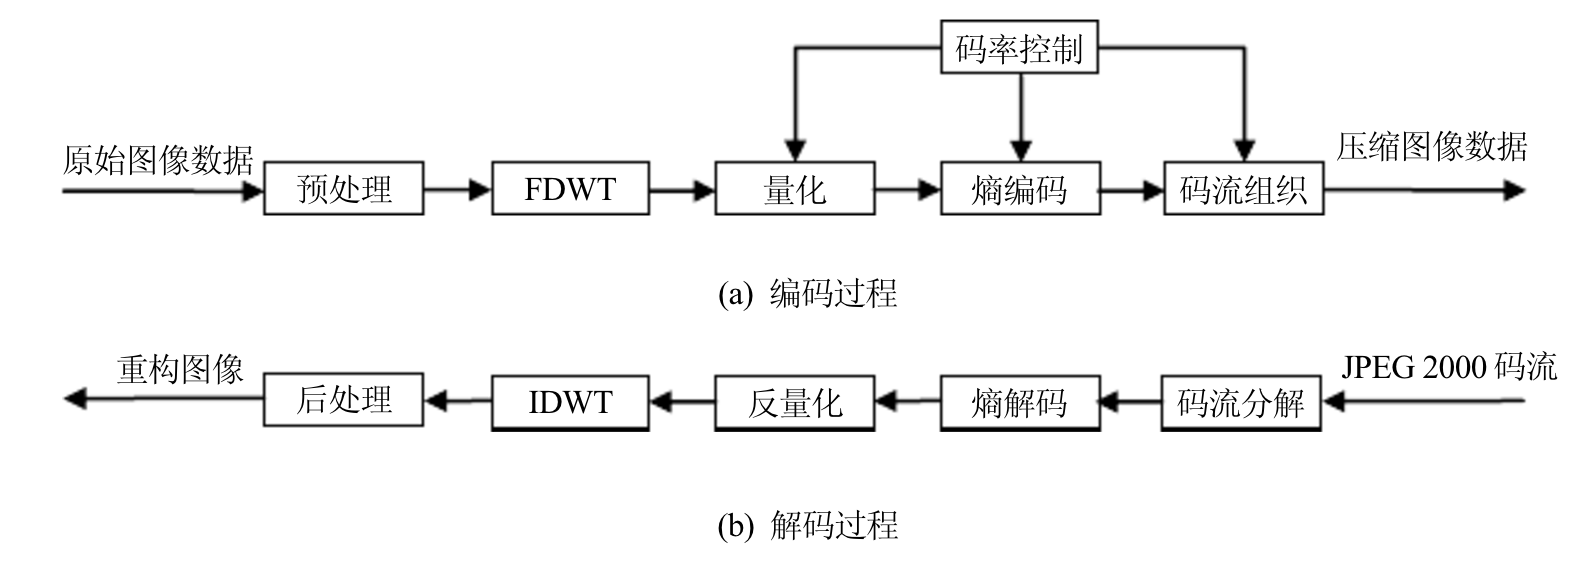
\includegraphics[scale=0.35]{b1}
	\caption{JPEG 2000核心编解码模块与过程.}
	\label{b1}
\end{figure}

小组分工如下:
\paragraph{张奕朗:} 图像分块,电平平移归一化,小波变换
\paragraph{陈幸豪:} 色彩分量变换,量化
\paragraph{高云帆:} EBCOT(最佳截断嵌入码块编码 ),算术编码,数据流
